
\documentclass{beamer}

% support unicode
\input glyphtounicode
\pdfgentounicode=1
\pdfmapfile{=cm-super-t2a.map}

% support specifically Russian
\usepackage{lmodern}
\usepackage[utf8]{inputenc}
\usepackage[T1,T2A]{fontenc}
\usepackage[english,russian]{babel}
\selectlanguage{\russian}


% STYLE
\usetheme{Malmoe}
\usecolortheme{default}
\useoutertheme{tree}

% Uncomment to remove nav
%\setbeamertemplate{navigation symbols}{}

% Code for section beginning
\AtBeginSection[]
{
	\begin{frame}
		\frametitle{План доклада}
		\tableofcontents[currentsection]
	\end{frame}
}



% Set picture materials
%\usepackage{graphicx} % note - beamer already imports
\graphicspath{ {../materials/img/} }



% META-INFO
\title{РАЗРАБОТКА И ПРИМЕНЕНИЕ МОДЕЛЕЙ MSVARX ДЛЯ АНАЛИЗА ЭКОНОМИЧЕСКИХ ЦИКЛОВ}
\author{Макаревич А.С.}
\institute[БГУ]{Белорусский Государственный Университет}
\date[Минск, 2018]{Минск, 2018}
\subject{text}


% 
\begin{document}


	% Title page
	\begin{frame}
		\titlepage
	\end{frame}

	\section{Описание задач}
		\subsection{Анализ экономических циклов}
		\begin{frame}
			\frametitle{Задача анализа экономических циклов}
			
			\begin{itemize}
				\item Базовый ряд -- Реальный ВВП РБ (цены 2014 г.)
				\item Экономический цикл (по НБЭИ США)
					\begin{itemize}
						\item объект: тренд ВВП
						\item фазы: <<рост>> и <<спад>>
						\item точки: <<пик>> и <<дно>>
					\end{itemize}
				\pause
				\item Опережающий индикатор -- Индекс Экономических Настроений (ИЭН)
					\begin{itemize}
						\item по данным сист. мониторинга предприятий НБ РБ
						\item циклы опережают ВВП на 4-5 месяца
					\end{itemize}
			\end{itemize}
			
		\end{frame}

		\subsection{Декомпозиция временных рядов}
		\begin{frame}
			\frametitle{Декомпозиция временных рядов}
			
			Сезонная декомпозиция - разложение ряда $y_t$ на компоненты:
			\begin{itemize}
				\item[$\tau_t$] тренд 
				\item[$c_t$] цикл 
				\item[$s_t$] сезонность 
				\item[$\varepsilon_t$] шум (irregular) 
			\end{itemize}			
		\end{frame}
	
		\begin{frame}
			\frametitle{Рассмотренные методы}
						
			\begin{itemize}
				\item Сезонная корректировка (X13-ARIMA-SEATS): тренд + цикл, сезонность, шум
				
				\item Фильтр Ходрика--Прескотта: 
					\begin{itemize}
						\item низкочастотный: тренд, цикл, шум
						\item высокочастотный: тренд (или цикл), шум
					\end{itemize}
				
				\item Метод Хамильтона: тренд + шум, цикл
			\end{itemize}
			
		\end{frame}
		
		\begin{frame}
			\frametitle{Результаты}
			
			TODO: Update image
			
			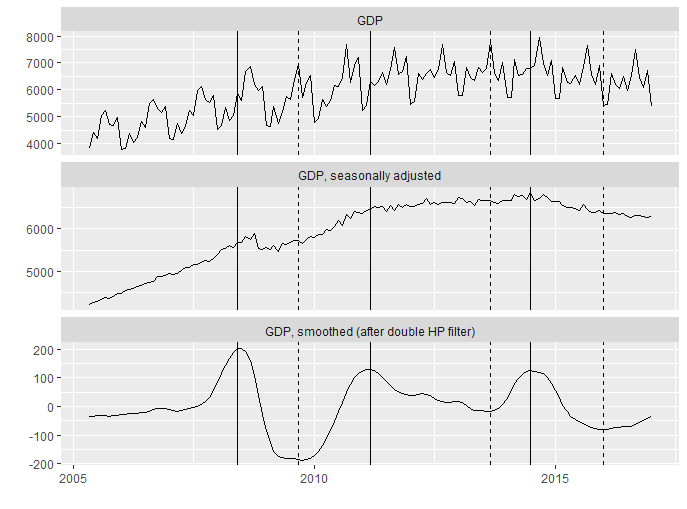
\includegraphics[height=0.7\textheight]{gdp_base-sa-hp}
		\end{frame}
		
		\subsection{Модели с переключением состояний}
		\begin{frame}
			\frametitle{Модели с переключением состояний}
			
			Режим -- состояние системы (например, фазы <<роста>> и <<падения>>).
			
			Каждому режиму соотносится своя построенная модель.
			
			Переключение режимов происходит по какому--то правилу. Из относительно простых -- независимое переключение ($IS$) и цепь Маркова ($MS$).
			
			В качестве базовой модели -- $ARX$, в кач. экзогенной -- ИЭН.
			
			$ \Rightarrow $ модель $ MS-ARX $
			
		\end{frame}
	
	\section{Экспериментальные исследования}
		\subsection{Моделирование с MS-ARX}
		\begin{frame}
			\frametitle{Результирующая модель MS-ARX}
			
			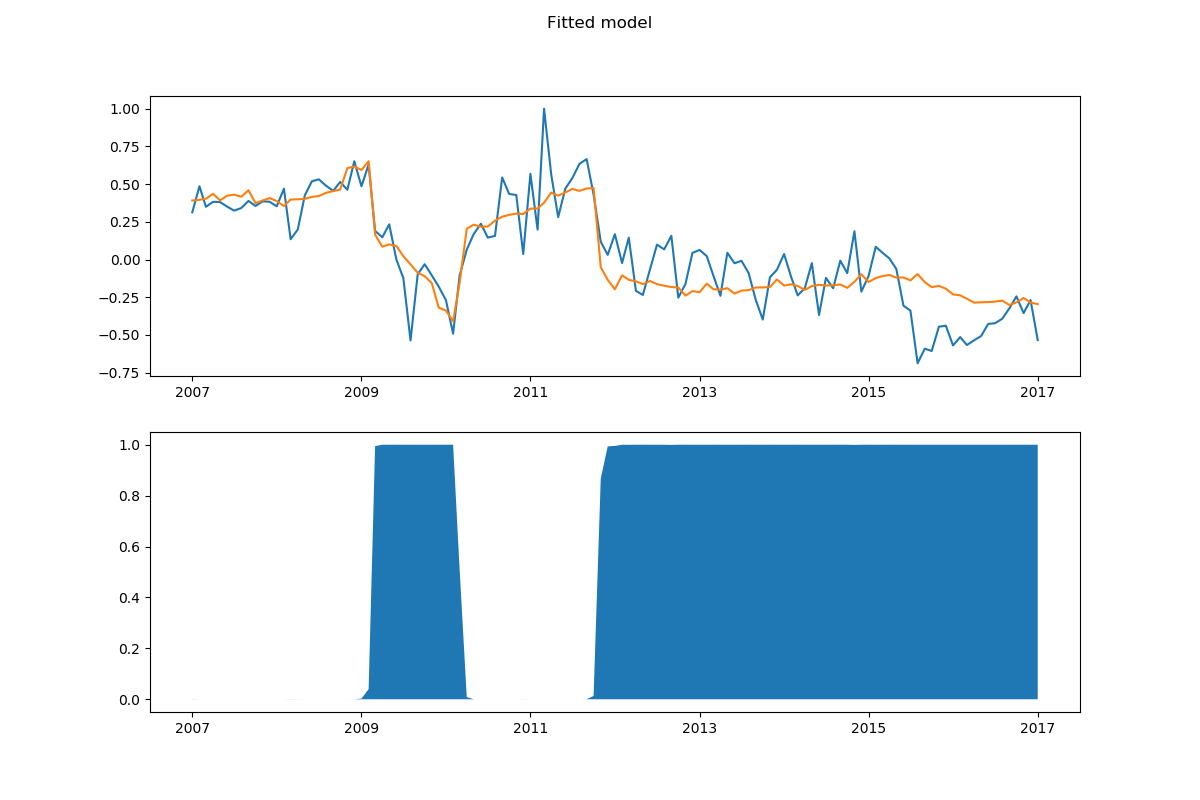
\includegraphics[height=0.8\textheight]{m0_fit}
			
			MS(2)-AR(0)X по рядам ВВП и ИЭН, скорр. по Хамильтону
		\end{frame}

		\subsection{Моделирование с MS-ARX}
		\begin{frame}
			\frametitle{Остатки модели MS(2)-AR(0)X
				\footnote{Модели с AR(1) не удовлетворяли критериям выбора модели: слишком много переключений режимов, либо незначимые коэфф.}
			}
			
			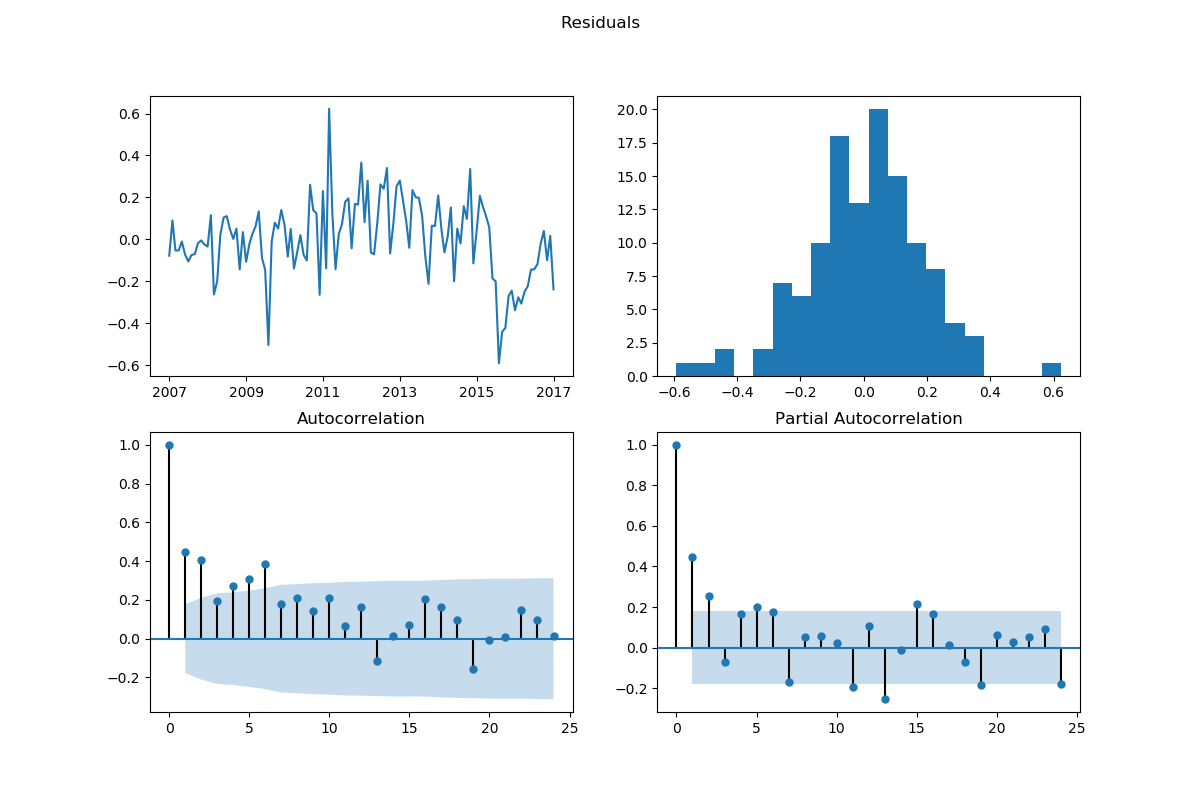
\includegraphics[height=0.8\textheight]{m0_resid}
		\end{frame}
	
	\section{Библиотека TS4DS}
		\begin{frame}
			\frametitle{Разработка библиотеки TS4DS}
			
			Разработана библиотека для анализа временных рядов ``Time Series for Data Science'' (TS4DS). 
			
			Главные результаты разработки:
			\begin{enumerate}
				\item Совмещены различные подходы к анализу данных (эконометрика, машинное обучение)
				\item Реализованы основные модели, трансформации, стат. тесты и т.д.
				\item Проведена автоматизация выбора моделей (auto-ARIMA)
			\end{enumerate}
		\end{frame}
		
		\begin{frame}
			\frametitle{Пример: Автоматизация выбора модели}
				
			TODO: maybe change to BY GDP example auto-ARIMA?
			
			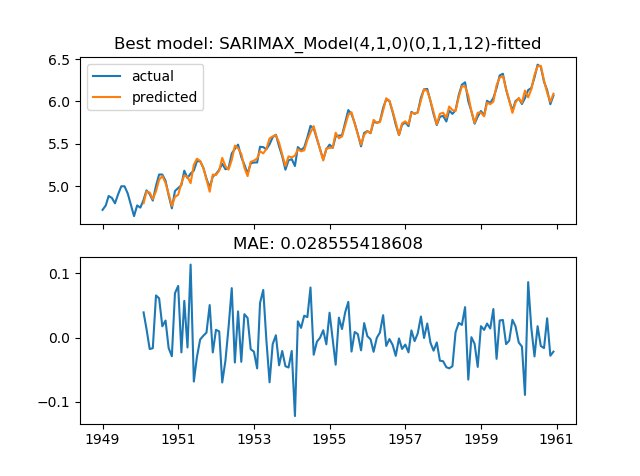
\includegraphics[height=0.8\textheight]{auto_sarimax}
		\end{frame}

		\begin{frame}
			\frametitle{Пример: Точность прогнозов}
			
			TODO: add numbers
			
			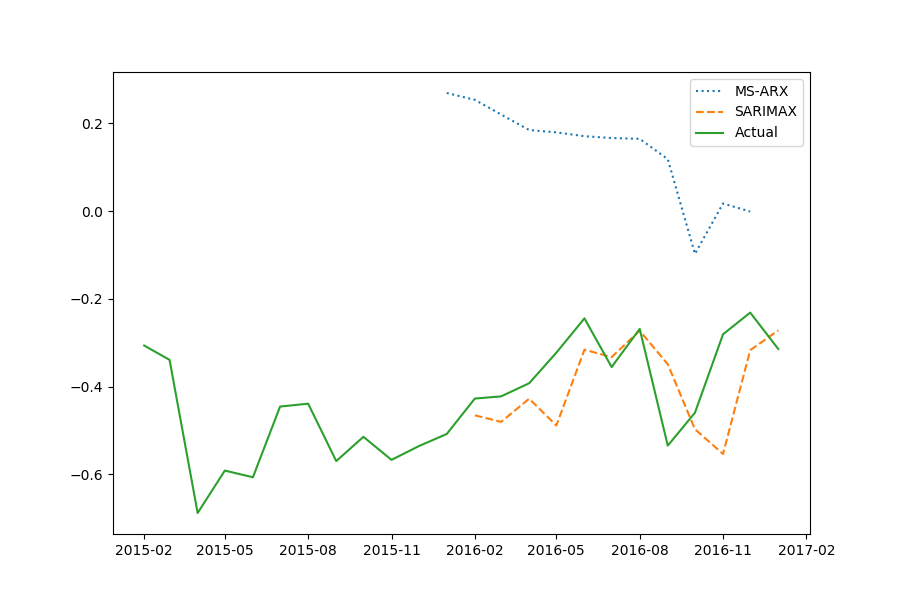
\includegraphics[height=0.8\textheight]{compare_ham}
		\end{frame}
		
	
	\begin{frame}[plain]
		\huge{Спасибо за внимание!}
	\end{frame}
	
\end{document}